\section{\tool{} Leakage Definition}
In the section, we discuss how \tool{} quantifies the amount of
leaked information. \tool{} is a dynamic-based approach to 
quantify the information leakage. We will first introduce 
the limitation of existing quantification metrics. After
that, we introduce the abstract and notation for the paper 
and propose our method.

\subsection{Problem Setting}
Existing static-based side-channel quantification works~\cite{182946,Wichelmann:2018:MFF:3274694.3274741 } define information leakage
using max entropy or Shannon entropy. These definitions provide a strong security guarantee
when trying to prove a program is secure enough if zero bit of information is leaked 
reported by their approaches. However, it is useless if the tool report the program leaks
some information. Moreover, those metrics does not apply to static method.


\begin{figure}[h!]
    \centering
\begin{lstlisting}[xleftmargin=.03\textwidth,xrightmargin=.01\textwidth]
uint_8 password = input();
if(password == 0x1b){
    pass();
}else{
    fail();
}
\end{lstlisting}
\caption{A dummy password checker}
\label{figure:password checker}
\end{figure}

Considering the example~\ref{background::side-channel}, if an attacker knows the
code executes branch $\{{1, 2\}}$ by side-channel attacks, the attacker can infer the total key size equals to 16. 
Without the above information, an attacker can only know $key[1]$ and $key[2]$ have 256*256 = 65536 
possibilities.
Suppose it is a dummy password checker, in which case the attacker can fully retrieve the password.
Therefore, the total information leakage should be 8 bits, which equals to the size
of unsigned char. 
According to the mutual definition, however, the leakage will be 1.7 bits. \fixme{use footnote or list the calculation process}. The maximal information
leakage is 2 bits. \fixme{the same with previous}. Both approaches fail to tell how 
much information is leaked during the execution precisely.

The problem with the existing methods is that they are static-based and the 
input values are neglected by the previous definition. 
They assume the attacker runs the program multiple times with many different sensitive 
information as the input. Both the mutual information and the max-leakage give an ``average" 
estimate of the information leakage. However, it isn't the typical scenario for an adversary to 
launch an side-channel attack. When a side-channel attack happens, the adversary wants 
to retrieve the sensitive information, in which case the sensitive information is fixed (e.g. AES keys). 
The adversary will run the attack over and over again and guess the value bit by bit. Like the 
previous example, the existing static method does not work well in those situations.

\begin{figure}
  \centering
   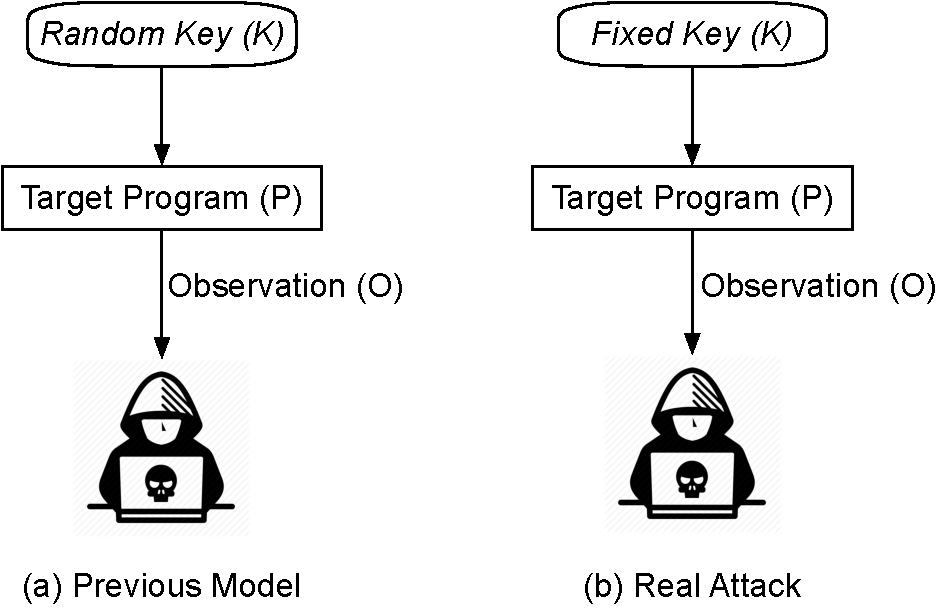
\includegraphics[width=.9\columnwidth]{./figures/RA.pdf}
   \caption{\fixme{some caption here}}
\end{figure}

\vspace*{6pt}

\subsection{Notations}
\subsection{Theoretical Analysis}
Suppose a program with some
sensitive input $K$, an adversary has some observations ($O$) by side channels.  
 %In this work, the observations are referred as the secret-dependent control-flows and
 %secret-dependent data-access patterns. 
  The conditional entropy $H(K|O)$ is
\begin{displaymath}
    H(K|O) = - \sum_{o_j {\in} O} {P(o_j) \sum_{k_i {\in} K}{P(k_i|o_j)\log_2P(k_i|o_j)}}
\end{displaymath}
Intuitively, the conditional information marks the uncertainty about $K$ after the adversary
has gained some observations ($O$). 

Some previous work uses the mutual information $I(K; O)$ to quantify the leakage which is defined 
as follows:
\begin{displaymath}
    \mathit{Leakage} = I(K;O) = \sum_{k_i {\in} K}{\sum_{o_j {\in} O}{P(k_i, o_j)\log_2\frac{P(k_i, o_j)}{P(k_i)P(o_j)}}}
\end{displaymath}
where $P(k_i, o_i)$ is the joint discrete distribution of $K$ and $O$.
Alternatively, the mutual information can also be computed with the following equation:
\begin{displaymath}
    \mathit{Leakage} = I(K;O) = H(K) - H(K|O) = H(O) - H(O|K)
\end{displaymath}

For a deterministic program, once the input $K$ is fixed, the program will have the same
control-flow transfers and data-access patterns. As a result, $P(k_i, o_j)$ will always
equals to 1 or 0. So the conditional entropy $H(O|K)$ will equal to zero. So the leakage defined
by the mutual information can be simplified into:
\begin{displaymath}
\label{mutual:information}
    \mathit{Leakage} = I(K;O) = H(O)
\end{displaymath}
In other words, once we know the distribution of those memory-access patterns. We can 
calculate how much information is actually leaked.

